\documentclass[12pt,halfparskip]{scrartcl}

\usepackage{../pystructure}

\begin{document}

\pagestyle{plain}

\section*{Structural Analyser for Python – Project Proposal}
\vspace{-0.5cm}

\emph{by Reto Schüttel \& Robin Stocker, 12th February 2008}

\vspace{0.2cm}

Planning and analysing a program's structure and internal dependencies is a common task when working on larger projects. Such analysis helps to meet the defined architectural design goals or to find structural flaws like cyclic dependencies. A clear architecture becomes more and more important as software grows.

The project's goal is to develop a structural analyser for programs written in the Python programming language. The analyser should be able to parse an application's source code and generate the following information:

\begin{itemize}
	\item Structure of the project including modules, classes and methods
	\item Dependencies between these components. For example when method \id{a} in class \id{A} calls method \id{b} in class \id{B}, there is a dependency from \id{A} to \id{B} and from \id{a} to \id{b}.
\end{itemize}

(1) The generated data can be used for various further analysis. Headway Software developed a program structure analyser (Structure 101g) which takes such a dependency graph and visualises it. The data is exchanged between the analyser and Structure 101g using XML files.

(2) Of course the dependency representation can be used for other purposes as well.

\begin{figure}[h] \centering
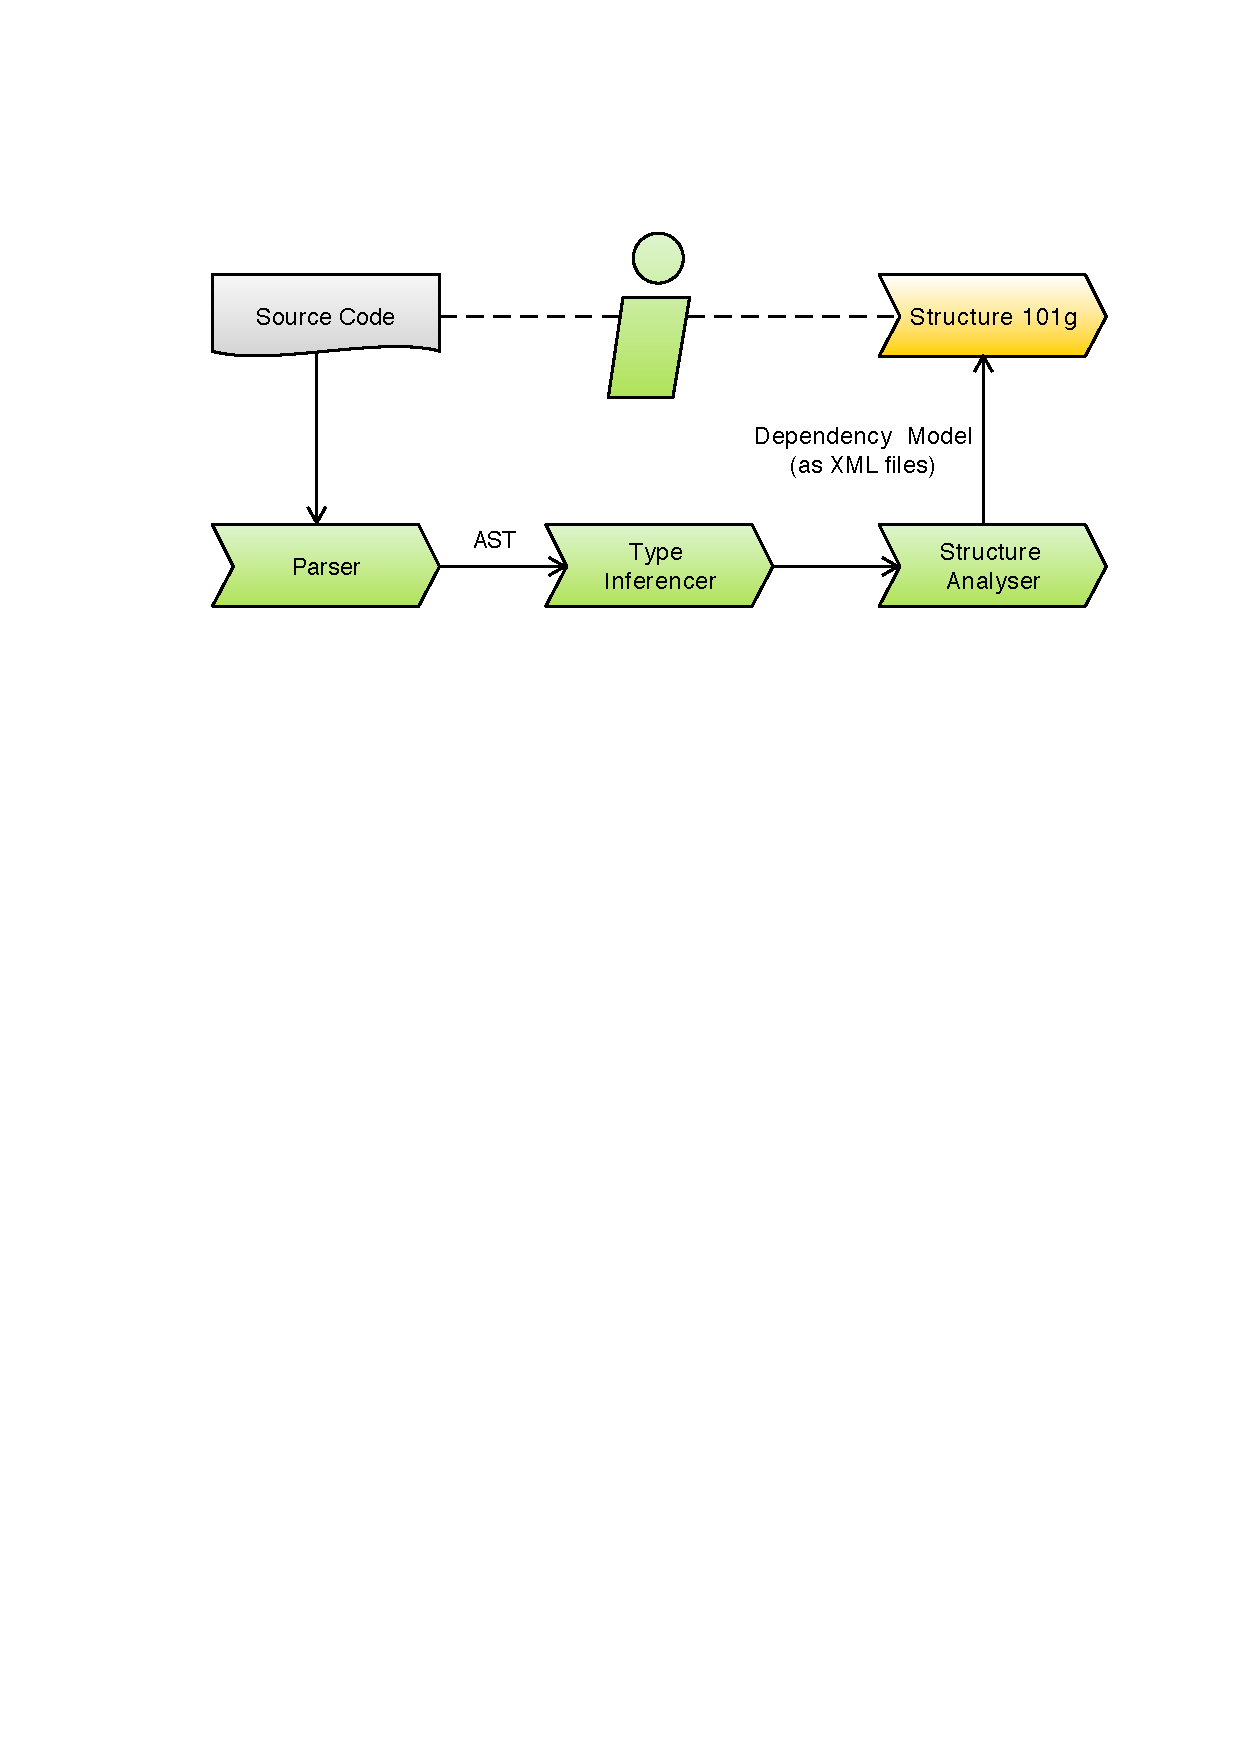
\includegraphics[width=0.75\textwidth]{big_picture}
\end{figure}

For Java, structural analysis has turned out to be a valuable instrument, but for Python these techniques are not (yet) used often. The project should do some research on this topic and try to answer the following questions:

\begin{itemize}
	\item Is structural analysis also helpful for dynamic languages like Python?
	\item Are existing Python projects even suitable for structural analysis?
	\item \ldots or does fulfilling the needs of the analyser require extensive care during the development?
	\item What's the Python community's opinion about structural analysis?
\end{itemize}


\end{document}
